\section{Stato dell'arte}
\label{ch:panoramica}

In questa sezione viene presentata un'analisi comparativa di alcuni dei più famosi sistemi di annotazione esistenti. Lo scopo di questa ricerca è quello di individuare i le caratteristiche comuni ai vari strumenti e le loro limitazioni. Da questa analisi è stata stilata una lista di requisiti che portano WATSS ad essere in accordo con gli altri sistemi introducendo allo stesso tempo nuove caratteristiche.

L'analisi dei sistemi si è incentrata principalmente su 3 strumenti open source esistenti: \emph{LabelMe}, \emph{ViPER-GT} e \emph{VATIC}. Per ciascuno dei sistemi è stata stilata una lista di caratteristiche offerte ed evidenziate le eventuali limitazioni. Infine è presentata un'analisi anche con il sistema WATSS.

\subsection{LabelMe}

\emph{LabelMe}\cite{Russell:2008:LDW:1345995.1345999} è un sistema Web che consente l'annotazione di oggetti all'interno di immagini. Le singole annotazioni sono effettuate mediante la definizione di aree poligonali nell'immagine e l'assegnazione di una label. Il tool offre la possibilità di indicare se un oggetto annotato è occluso o meno da altri oggetti presenti nella scena (non consente però di individuare la parte occlusa o visibile).

Le annotazioni possono essere annidate, è possibile dunque etichettare oggetti che sono inclusi gli uni negli altri. 

In aggiunta alle annotazioni di oggetti il sistema consente di annotare intere aree dell'immagine: questo è reso possibile andando inizialmente a delimitare una porzione di immagine ed associando ad essa una label. In questo caso l'area così definita viene colorata interamente ed è necessario stabilire se si tratta di un'area interna o esterna.

\begin{figure}[H]
\centering
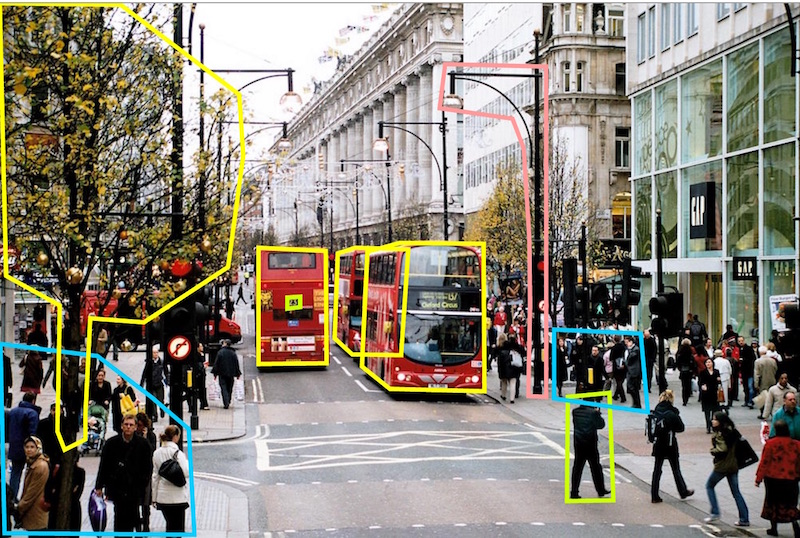
\includegraphics[width=0.6\linewidth]{images/labelme.jpg}
  \label{fig:labelme}
  \caption{Annotazione di un'immagine tramite LabelMe}
\end{figure}

In fase di esportazione delle annotazioni viene generata una struttura in formato XML che è possibile importare nuovamente in un'altra immagine.

Il sistema non prevede la possibilità di generare \emph{proposals} per le annotazioni, tutto il lavoro è a carico dell'utente.

\subsection{ViPER-GT}

\emph{ViPER-GT}, acronimo di \emph{Video Performance Evaluation resource}, è un sistema di annotazione per video e la generazione di un \emph{groundtruth}. 

Il sistema consente di annotare un video indicando cosa è contenuto nella scena, definendo un insieme di \emph{classi} per ciascuna tipologia di contenuto. L'annotazione avviene manualmente da parte dell'utente che definisce delle \emph{bounding boxes}, regioni di interesse dell'immagine, andando ad associare a ciascuna di esse una classe di appartenenza ed alcune metadati aggiuntivi, come ad esempio titolo, dimensione, etc. Le regioni possono essere di forme diverse: cerchi, ellissi, rettangoli e generici poligoni (definiti dai loro vertici).

\begin{figure}[h]
\begin{center}
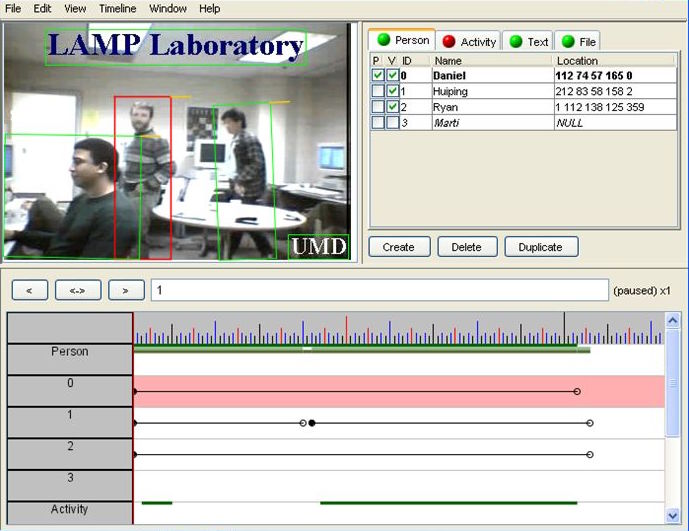
\includegraphics[width=0.3\textwidth]{images/vipergt.jpg}
\end{center}
  \caption{Interfaccia utente del tool ViPER-GT}
\label{fig:vipergt}
\end{figure}


Le annotazioni effettuate vengono visualizzate in una \emph{timeline}: allo scorrere dei frame le annotazioni presenti nella scena corrente vengono evidenziate.

Il tool mette a disposizione anche un sistema di predizione delle annotazioni inserite basato sull'interpolazione lineare delle bounding boxes di più frame consecutivi. Questo metodo risulta molto efficace se si fornisce un numero di annotazioni, \emph{ancore}, adeguato; con poche ancore definite la predizione risulta essere molto approssimativa.

\subsection{VATIC}

VATIC\cite{Vondrick:2013:ESU:2436010.2436013} è un software di annotazione di video distribuito ai fini della ricerca nell'ambito della Computer Vision che consente la creazione di grandi dataset video. Il tool utilizza il sistema di crowdsourcing \emph{Mechanical Turk} di Amazon.

Il sistema consente l'inserimento manuale di annotazioni per ciascun frame del video, definite mediante delle bounding box rettangolari. 

Il tool dispone di una serie di plugin aggiuntivi che ne aumentano le potenzialità:
\begin{itemize}
\item \emph{Tracking integration} per il tracciamento di oggetti in movimento nella scena
\item \emph{Sentence annotation} per l'annotazione di frasi e parole
\item \emph{Labeling time intervals} per l'annotazione di intervalli temporali
\item \emph{Human action labeling} per l'annotazione di azioni umane nella scena
\end{itemize}

\begin{figure}[h]
\centering
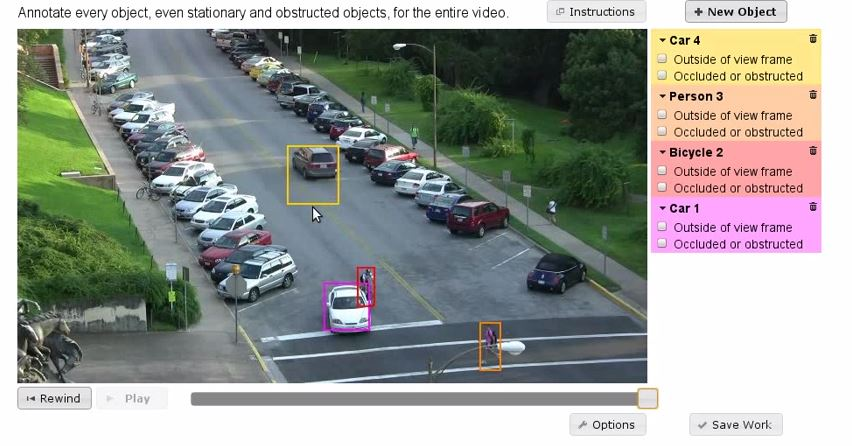
\includegraphics[width=0.6\linewidth]{images/vatic.jpg}
  \label{fig:vatic}
  \caption{Interfaccia utente del tool VATIC}
\end{figure}

Il tool è pensato principalmente per l'\emph{object detection} nelle scene.

\subsection{WATSS}

WATSS\cite{Bartoli:2015:WWA:2733373.2807411}, \emph{Web Annotation Tool for Surveillance Scenarios}, è un sistema web per l'annotazione di dataset. Il tool è stato sviluppato per consentire l'annotazione del dataset \emph{MuseumVisitors}\cite{bartoli2015museumvisitors} come parte del progetto MNEMOSYNE e rilasciato successivamente open source.

Il tool permette l'annotazione di persone e oggetti nella scena mediante la definizione di bounding boxes. In caso di occlusione è possibile poi indicare, mediante la definizione di una seconda bounding box, la parte visibile della persona o oggetto annotati.

\begin{figure}[h]
\centering
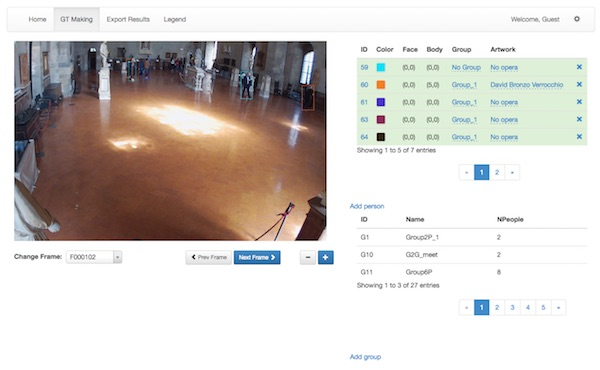
\includegraphics[width=1\linewidth]{images/watss.jpg}
  \label{fig:watss}
  \caption{Interfaccia utente del tool WATSS}
\end{figure}

A ciascuna annotazione corrisponde un'\emph{identità}: della persona annotata viene generato un avatar che consentirà di annotare la stessa persona negli altri frames del video.
Per ciascuna annotazione è inoltre possibile indicare inoltre l'\emph{orientazione del volto e del corpo} e il \emph{punto di interesse} presso cui si trovano nella scena (nel caso del museo i punti di interesse sono rappresentati dalle varie opere d'arte).

In caso di presenza di gruppi di persone, è possibile indicare il gruppo di appartenenza definendo il nome dello stesso, così da poterle poi riassociare in seguito anche nelle altre camere.

Il tool consente l'annotazione da parte di più utenti e la gestione di più camere.
